\section*{Lezione 17}
\addcontentsline{toc}{section}{Lezione 17}

\subsection*{AES}
\addcontentsline{toc}{subsection}{AES}

La competizione degli anni '90 viene vinta da Rijndael e il suo AES, esso diventa standard dal 2002. Cifra blocchi di 128 bit per volta e le chiavi possono essere di diverse lunghezze (AES-128, AES-192 e AES-256). \'E più efficiente di DES e la sua implementazione software è più semplice.
Per semplicità vediamo solo AES-128, ma gli altri cambiano solo su pochi dettagli.
\begin{itemize}
	\item \textbf{Cifratura}: l'algoritmo opera su una matrice di stato 4x4 di 16 bytes (128 bits). Inizialmente la matrice contiene il blocco del messaggio in chiaro (riempita per colonne).\\
	Vengono generate le chiavi derivate e si effettua uno XOR fra i bit della matrice e quelli della \textbf{Roundkey}.
	Per nove volte (ogni chiave derivata) si effettuano queste operazioni:
		\begin{enumerate}
			\item \textbf{SubBytes} (sostituzione dei byte utilizzando una S-box)\\
			Essa è una operazione invertibile ma non lineare. Si fissa $b=(b_7,b_6,...,b_0)$ e si definiscono:
			\begin{figure}[h]
				\centering
				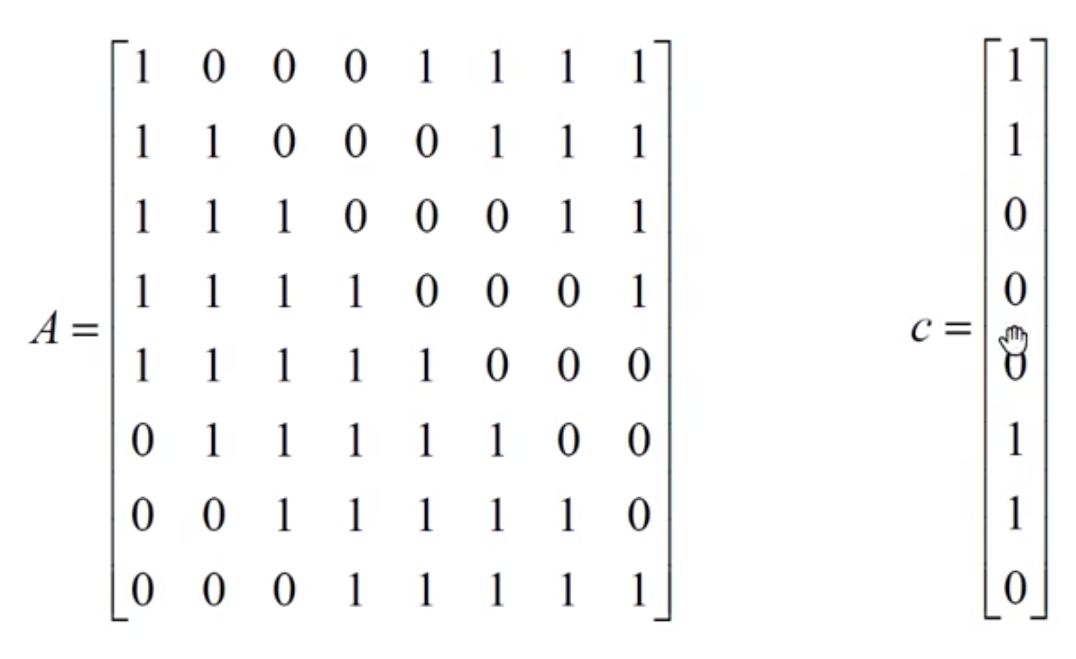
\includegraphics[width=0.7\linewidth]{immagini/img35}
			\end{figure}
			Poi, se $b\neq 0$ allora $b=b^{-1}$ e si ritorna $A \cdot b + c$.\\
			La non linearità sta nel calcolo dell'inverso di $b$ (resistenza ad attacchi ad approssimazione). Vedo i termini di $b$ come i coefficienti di un equazione di settimo grado ($b_7x^7 + b_6x^6 + \dots + +b_1x + b_0$), poi faccio la divisione con resto con il polinomio irriducibile $x^8+x^4+x^3+x+1$ nel campo $GF(2^8)$ ovvero con resto 0 o 1. In questo campo ci sono vettori di 8 elementi, la somma è lo xor, il prodotto poi si divide per lo stesso vettore.
			
			
			
			
			\item \textbf{Shiftrows} (rotazione delle righe)\\
			La prima riga rimane alterata, la seconda la terza e la quarta viene ruotata di 1, 2, 3 posizioni rispettivamente
			
			\item \textbf{MixColumns} (operazioni sulle colonne)\\
			Moltiplica ogni colonna per una matrice fissata e che diventa la nuova colonna.
			
			\item \textbf{AddRoundKey} (come prima, si effettua uno xor)
		\end{enumerate} 
		
	Come si generano le chiavi derivate? Spieghiamo per AES-128.
	Bisogna ottenere 11 chiavi, ognuna di 16 bytes. L'algoritmo lavora su parole di 4 bytes, quindi dobbiamo ottenere 44 parole che inseriamo in un array $w[0,..43]$. Si definiscono 10 costanti $Rcon[1]$, $Rcon[2]$, ..., $Rcon[10]$. Successivamente si segue questo pseudocodice:
	
		\begin{figure}[h]
		\centering
		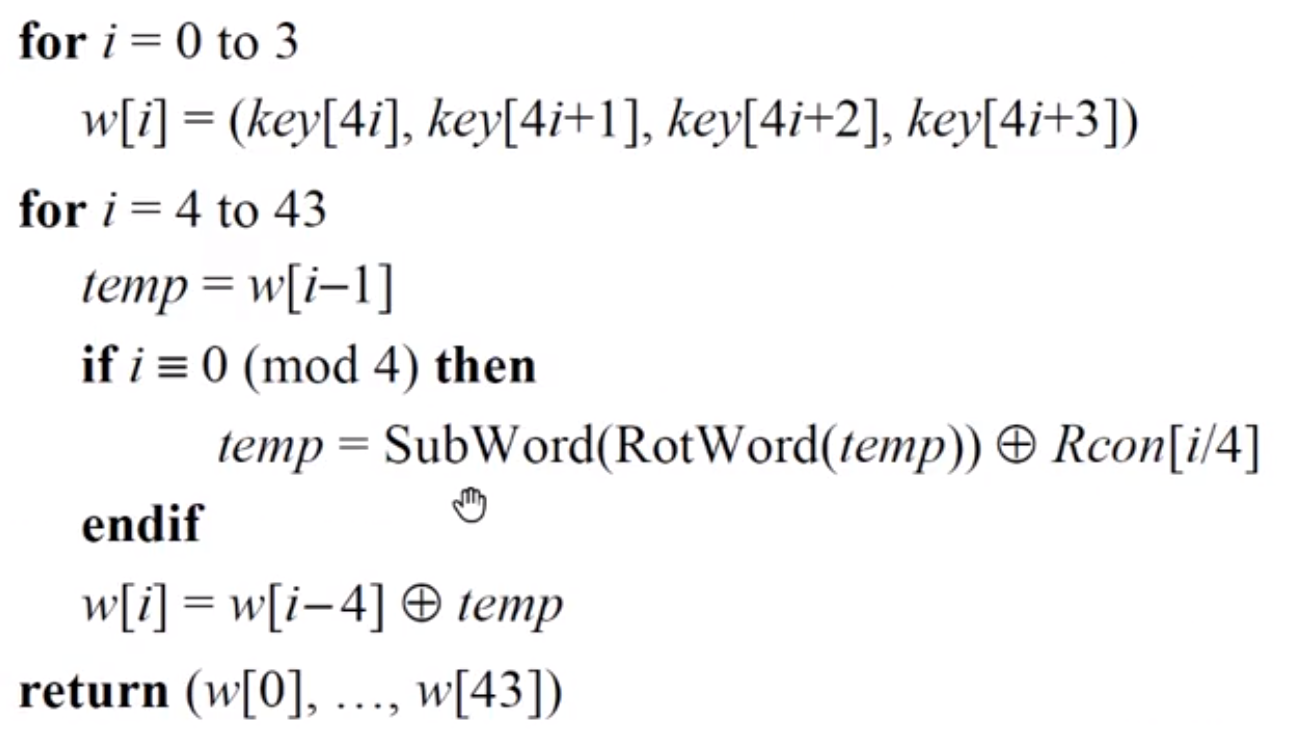
\includegraphics[width=0.9\linewidth]{immagini/img36}
	\end{figure}

\subsection*{Crittosistemi simmetrici}
\addcontentsline{toc}{subsection}{Crittosistemi simmetrici}

Abbiamo una sequenza di testi di in chiaro $m_1, m_2, ...$ e una chiave iniziale $k$, vogliamo avere una sequenza di testi cifrati $c_1, c_2,...$.\\
\textbf{Modi di operazione}: 
\begin{itemize}
	\item ECB (Electronic CodeBook)\\
	\begin{figure}[h]
		\centering
		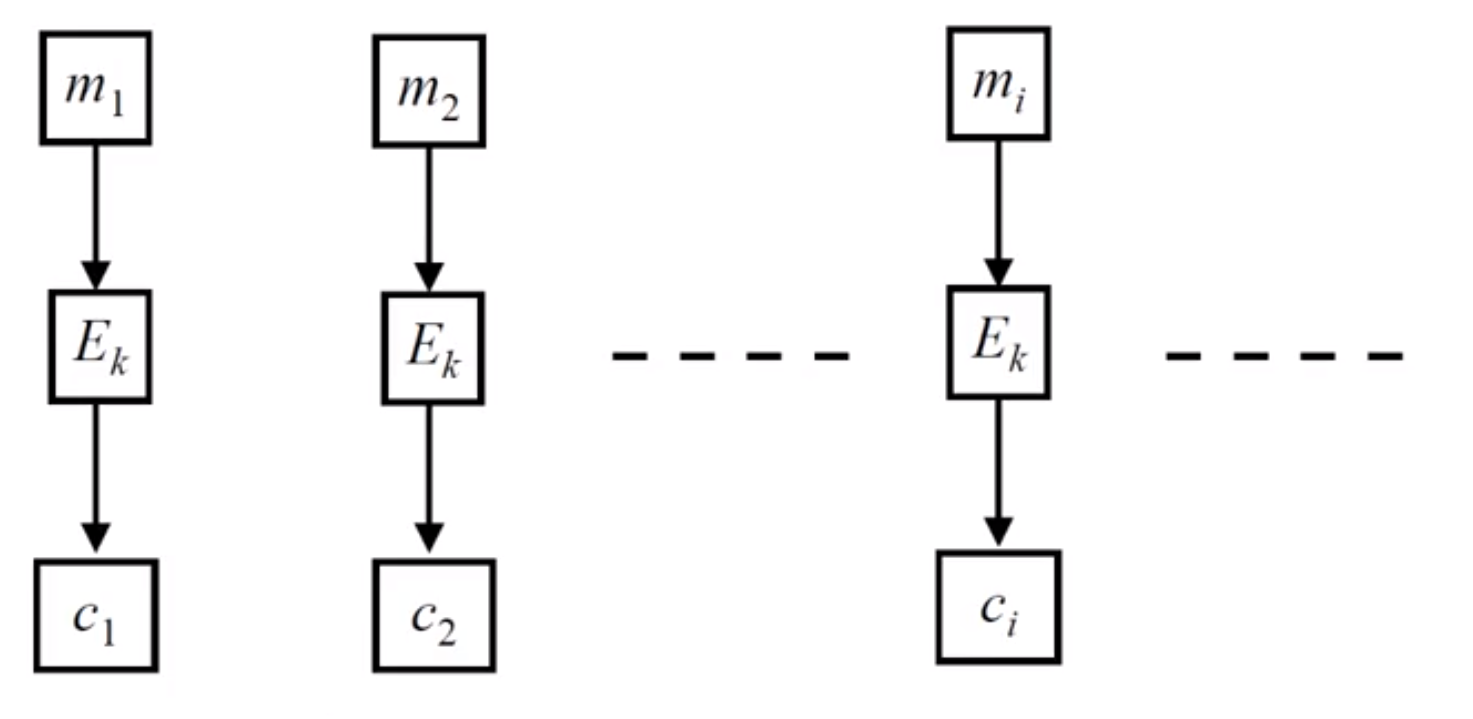
\includegraphics[width=0.5\linewidth]{immagini/img38}
	\end{figure}
	Il più semplice, ma anche il meno sicuro: ho $m_1$, lo cifro usando l'algoritmo $E_k$ e ottengo $c_1$ (e così via per tutte le $m$). Quando Eve comincia ad ascoltare (mettiamo che si perda alcuni pezzi), non ha vita difficile visto che ogni operazione di cifratura è indipendente dalla precedente. Oppure esempio pinguino Linux, cifro blocchi uguali in modo uguale, il risultato sarà strano ma avrà la forma del pinguino (il pattern non viene rotto). Ha però vantaggi: la modifica di un blocco di codice a causa del rumore, non rovina i successivi (adatto quindi a canali rumorosi).
	\item CBC (Cipher Block Chaining)\\
	\begin{figure}[h]
		\centering
		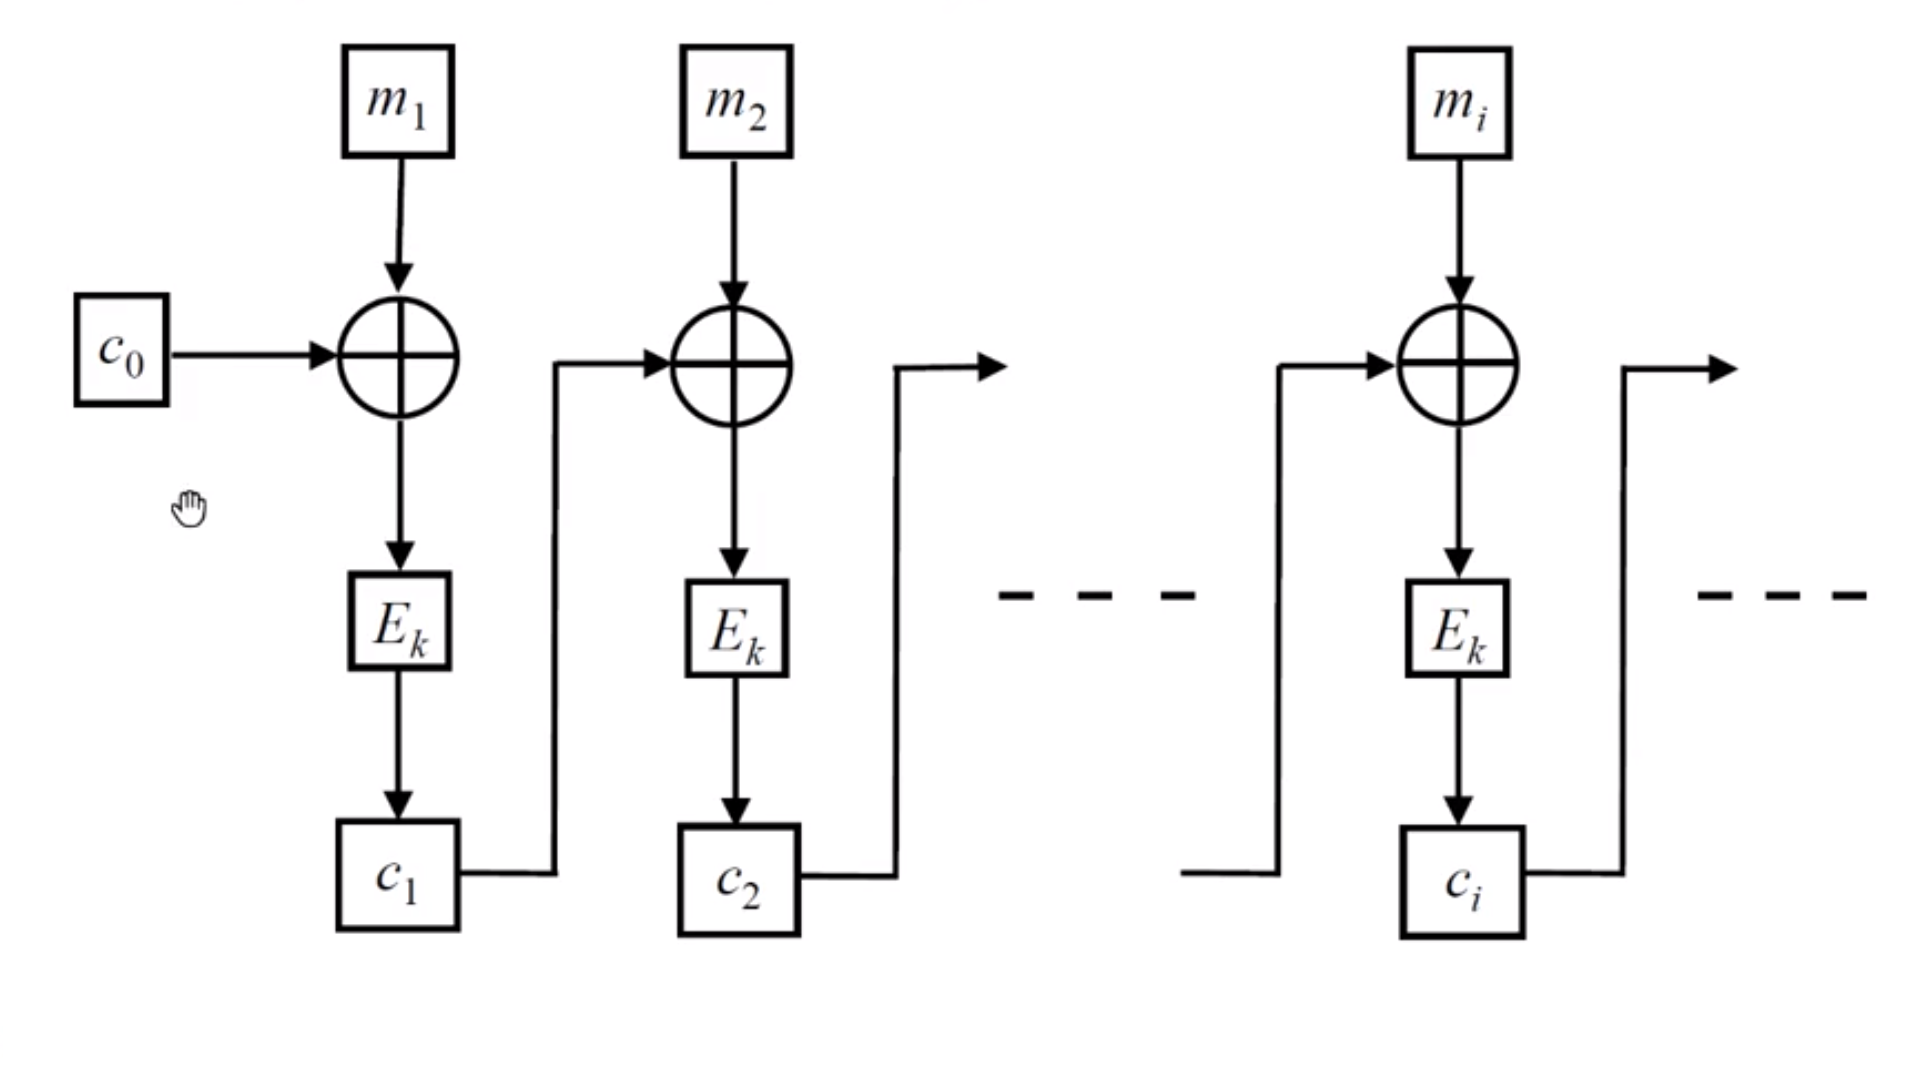
\includegraphics[width=0.5\linewidth]{immagini/img37}
	\end{figure}
Effettua una concatenazione con quello che è successo in precedenza. In particolare il messaggio cifrato $c_i = E_k(c_{i-1} \oplus m_i)$.
\'E il modo di operazione più usato (se cifri l'immagine del pinguino viene un casino). Il problema è che se il rumore rovina un blocco allora tutti i successivi verranno sbagliati. Quindi il canale di comunicazione dev'essere affidabile.
\item OFB (Output Feedback)\\
\begin{figure}[h]
	\centering
	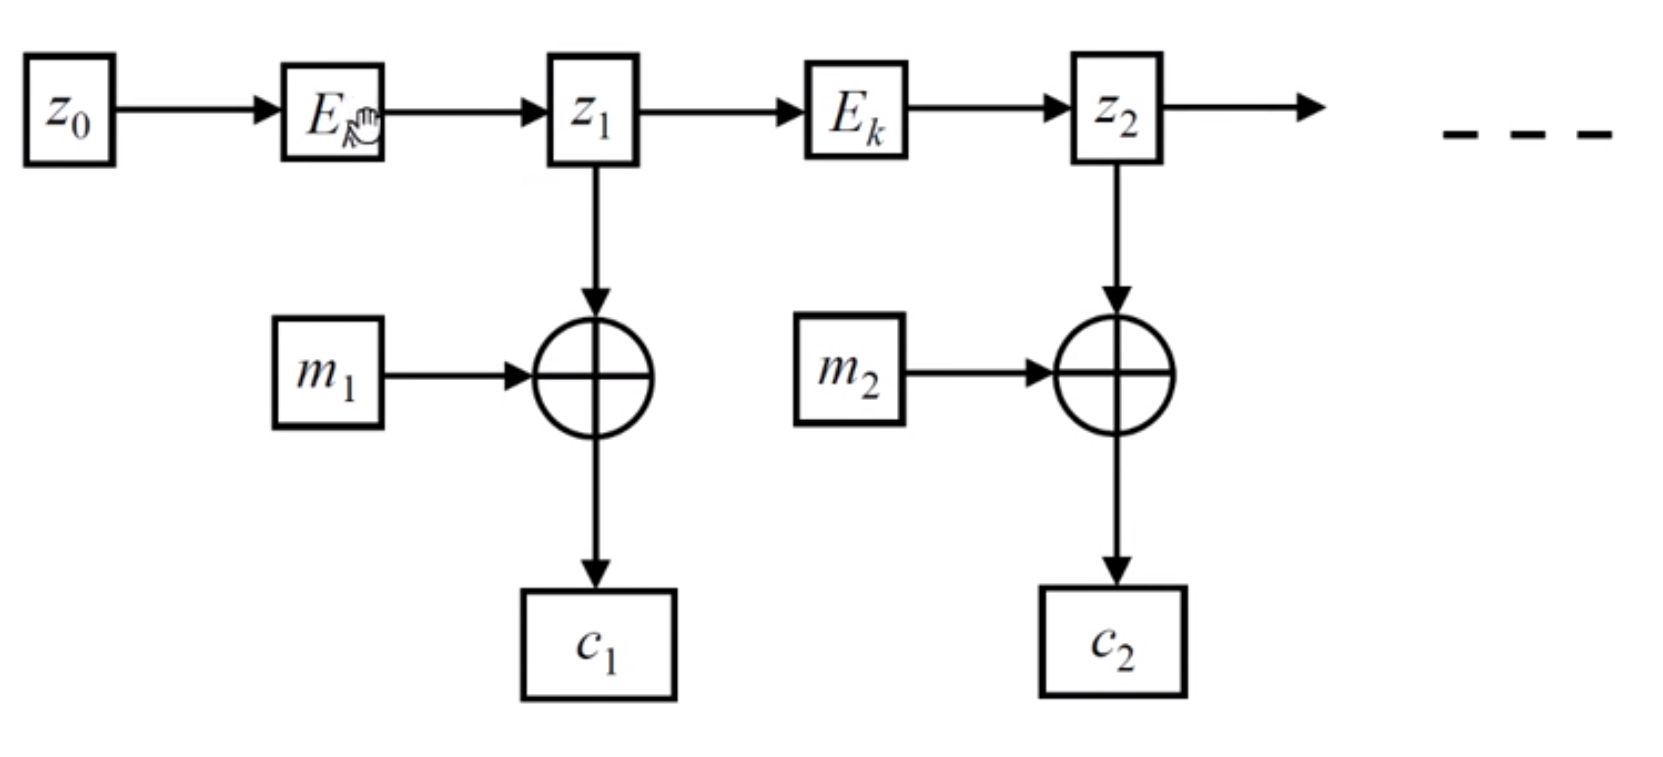
\includegraphics[width=0.5\linewidth]{immagini/img39}
\end{figure}
Viene prodotta una sequenza di chiavi derivate, che vengono utilizzate per effettuare la cifratura. In pratica cifro $m_1$ facendo lo xor con $z_1$ e così via. L'idea è fare lo xor con dei bit casuali per ottenere un risultato casuale. Parto da $z_0$ che trovo in maniera casuale. Se $E_k$ è fatto bene lo posso usare come generatore di numeri casuali.
Questo modo è molto veloce in quanto fa solo lo xor con le chiavi derivate (es guardo un video in HD). \'E affidabile anche in canali rumorosi in quanto l'aver perso un blocco $m_i$ non pregiudica quello successivo. Però è vulnerabile ad un attacco che modifica lo stream. (es. se si parla di cifre, prezzi, posso invertire un numero).
\item CFB (Cipher FeedBack)\\
\begin{figure}[h]
	\centering
	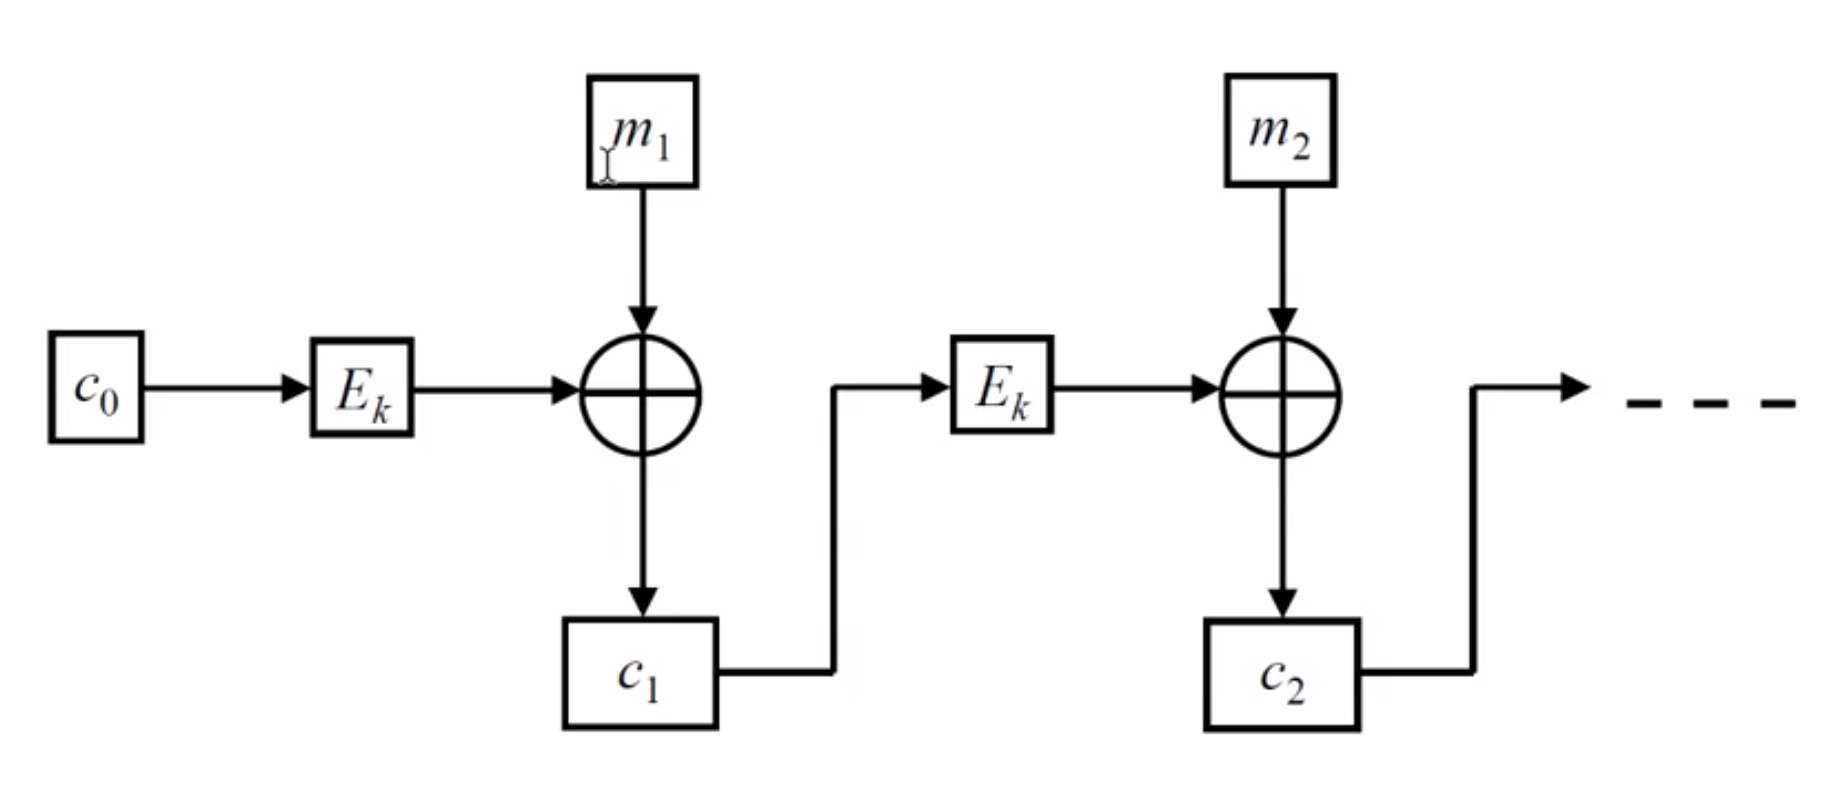
\includegraphics[width=0.5\linewidth]{immagini/img40}
\end{figure}
I blocchi del testo vengono cifrati facendo uno xor bit a bit con l'output dell'algoritmo di cifratura applicato al blocco precedente. Il canale dev'essere affidabile. Di pro c'è che se l'ultimo blocco arriva corretto allora anche i precedenti lo sono stati.

\newpage
\item s-bit CFB\\
\begin{figure}[h]
	\centering
	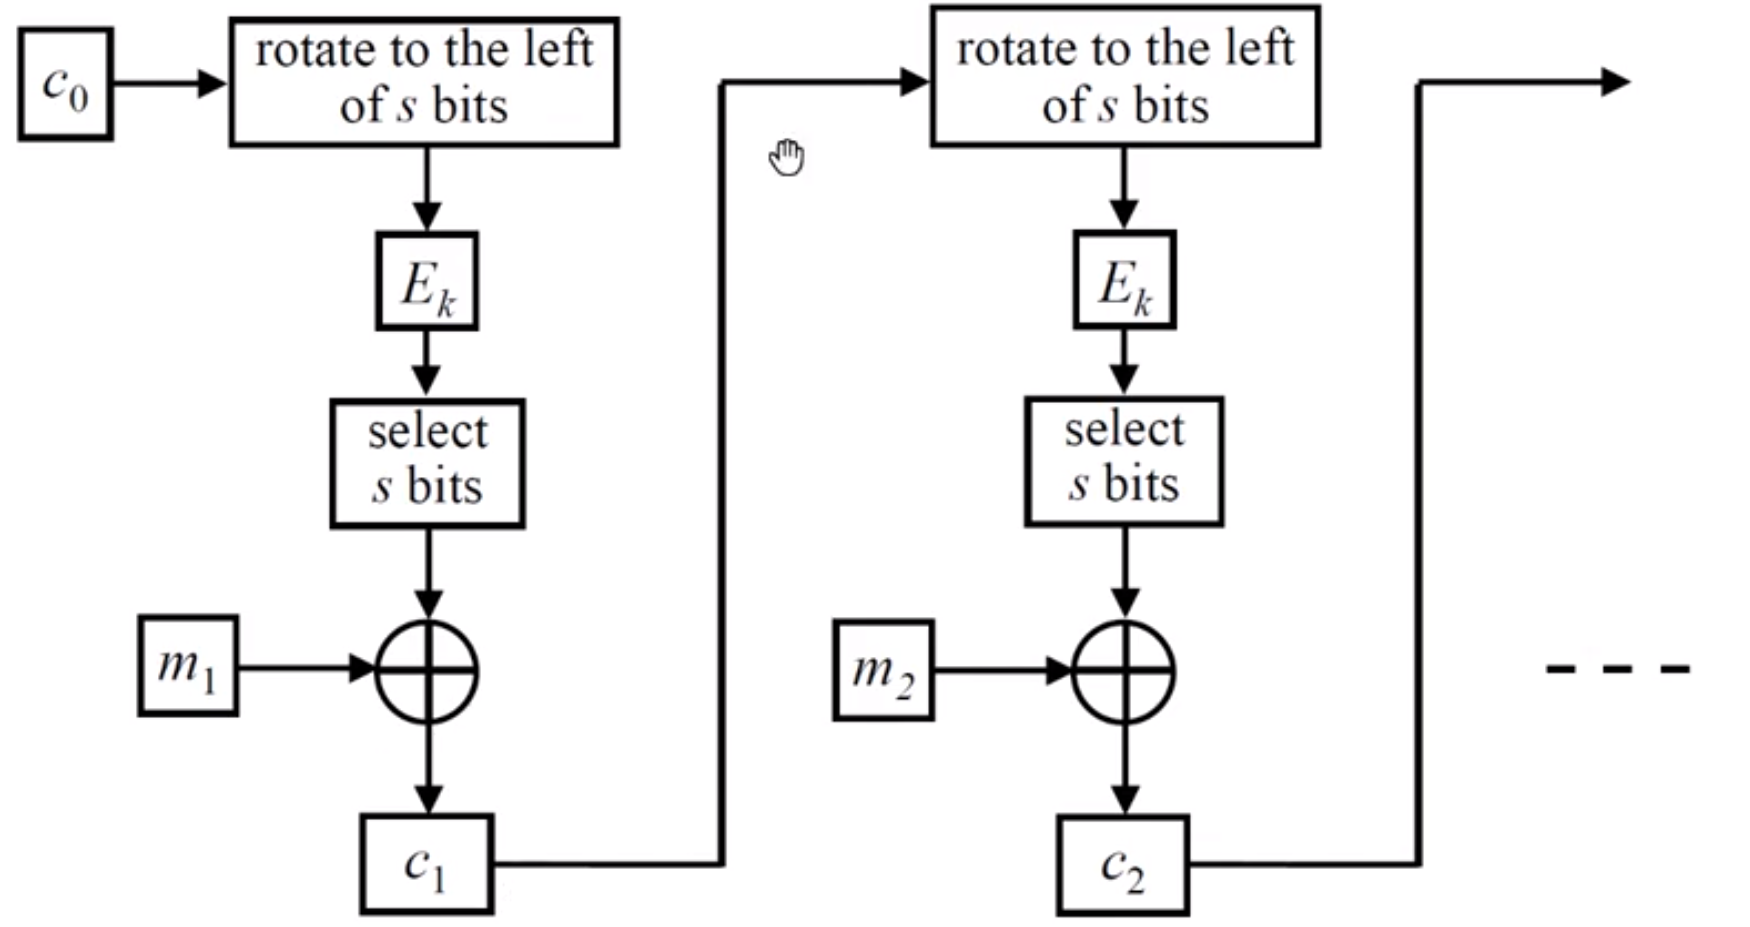
\includegraphics[width=0.5\linewidth]{immagini/img41}
\end{figure}
Funziona come CFB, però si applicano delle trasformazioni in più (rotazioni e selezioni). Però più lento.

\item CTR (Counter Mode)\\
\begin{figure}[h]
	\centering
	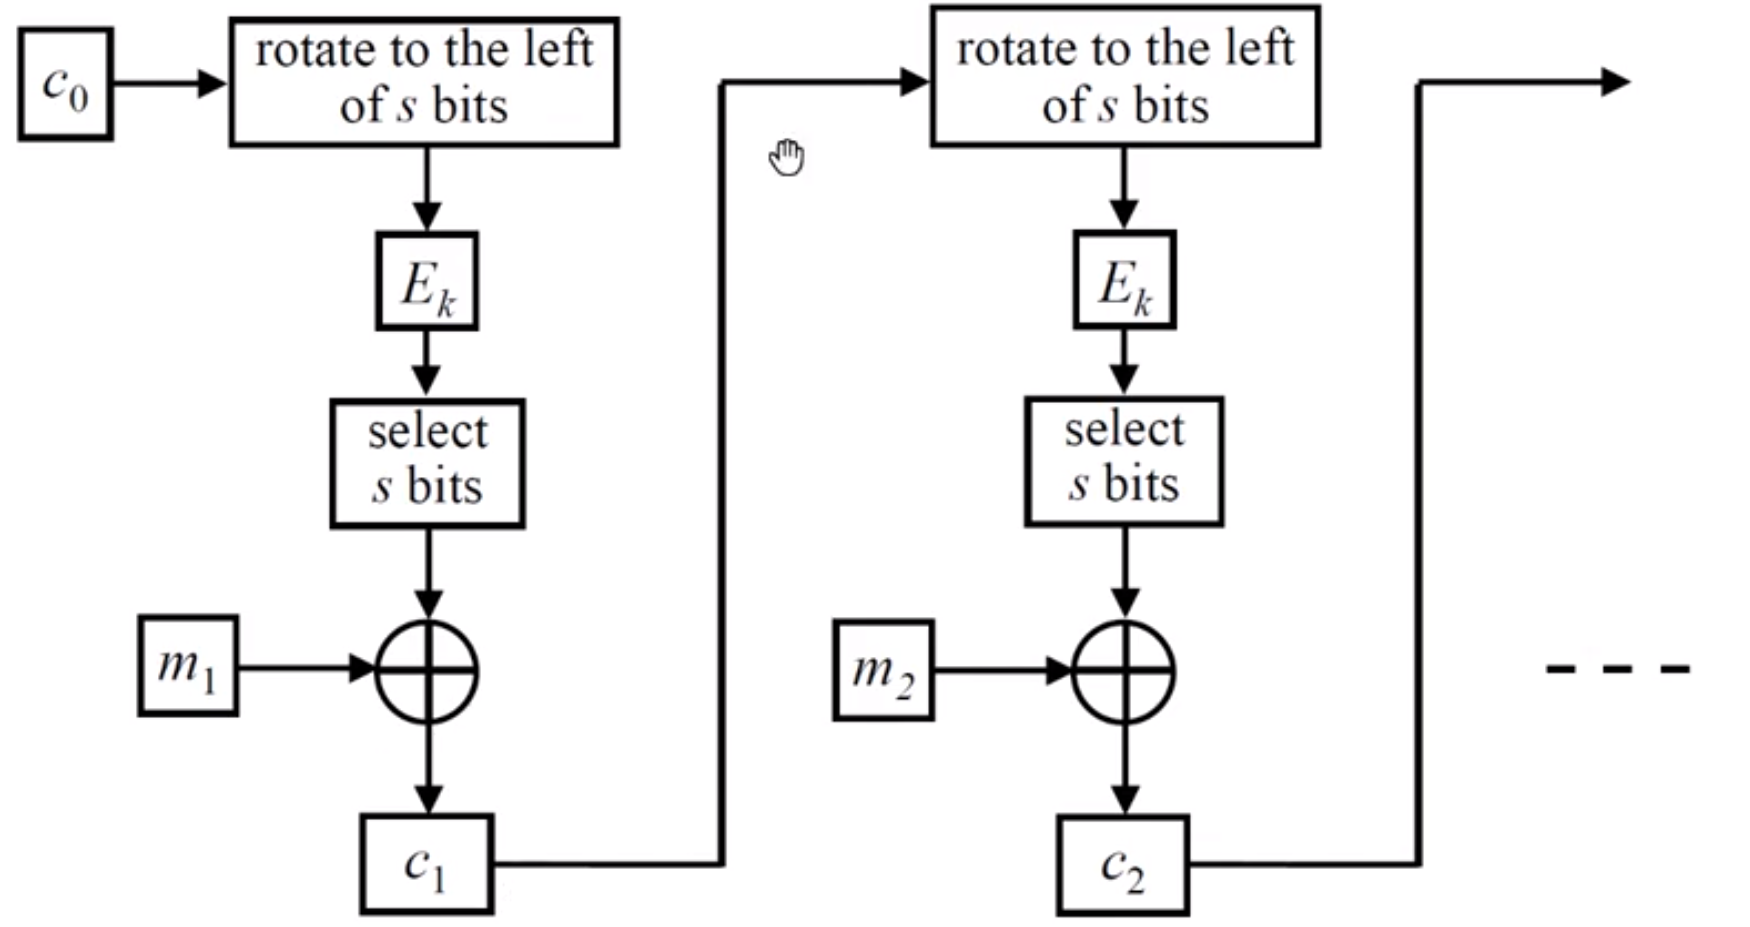
\includegraphics[width=0.5\linewidth]{immagini/img41}
\end{figure}
Usato dalle ATM (Asynchronous Transfer Mode) (es. Fastweb), ma anche da IPSec (VPN).
Si generano chiavi derivate diverse sfruttando i diversi valori dei contatori. Molto efficiente


\end{itemize}


	
\end{itemize}
